\section{Hashing}
To make Maths people feel better about this exam, with the courtesy of Harald Räcke.

The purpose of hashing is having a data structure that tries to directly compute the memory location from the given key, obtaining constant search time. 

Hash functions and their associated hash tables are used in data storage and retrieval applications to access and store information thanks to their efficiency.

Given an universe $U$ of keys and a set $S \leq U$ of used keys to be distributed over an array $T[0, \dots, n-1]$, an optimal hash function $H : U \rightarrow [0, \dots, n-1]$ should be fast to evaluate, have small storage requirements and a good distribution of elements over the whole table.

Ideally, the hash function would map all keys to different memory locations (direct addressing), yet this is unrealistic since the size of the table would be much larger than available memory.

Knowing previously the set $S$ of actual keys, it could be possible to design a simple function that maps all of them to different memory locations (perfect hashing); but this is not often the case.

The best expectation would be a function which distributes keys evenly across the table, yet this leads to the problem of collision: usually the universe $U$ is much larger than the table size $n$, hence there may be two elements $k_1, k_2$ from the same set $S$ so that $h(k_1) = h(k_2)$, and therefore getting mapped to the same memory location.

Typically, collisions do not appear once the size of the set $S$ of actual keys get close to $n$, but otherwise the probability of having a collision when hashing $m$ elements under uniform hashing is at least:
$$1 - e^{-\frac{m(m-1)}{2n}} \approx 1 - e^{-\frac{m^2}{2n}}$$

Practically, hash tables should be larger than the amount of keys to store, for instance the next power of two. There also are scaling coefficients such as 1.5 or 1.5, to avoid resizing too much and wasting space. Precomputing prime numbers is an useful option, but requires a range of about 10\% more than the number of keys.

There are methods to deal with collisions: open addressing, hashing with chaining, or just not resolving them at all.

Hashing with chaining arranges elements that map to the same position in a linear list, inserting at the front of the list. The average time required for an unsuccessful search is $A^- = 1 + \frac{m}{n}$, while for a successful search it is $A^+ \leq 1 + \frac{\nicefrac{m}{n}}{2}$.

Open addressing, in particular, stores all objects in the table defining a function that determines the position through a permutation of all possible $n - 1$ values. If an insertion fails, a new position is searched (either through a different function or looking for the first free slot).

A good choice for $h(i, j)$ to have an uniform distribution over the possible values is a modulo with a prime number.

Introducing prime numbers is relevant because the size of hash table should not have factors in common with the linear component of the function, otherwise keys would be mapped to the same position. Increasing has also to be done by odd numbers, to reduce the possibility of remainder zero.

Prime numbers can be generated through algorithms, of which the most basic is the prime sieve: a list of integers up to a desired number is created, and composite numbers are progressively removed until only primes are left. 

For large primes used in cryptography, a random chosen range of odd numbers of the desired size is sieved against a number of relatively small primes, and the remaining are subject to primality testing (Miller-Rabin).

To keep uniformity of the distribution even allowing new elements to be added, rehashing might be necessary, or incremental of the prime.

\subsection{Fibonacci hashing}
Fibonacci hashing is a variation of classic hashing using instead of a modulo operation, a multiplication by the golden ratio:
$$\frac{x}{y} = \frac{x + y}{x} \implies \phi = \frac{1 + \sqrt{5}}{2}$$

The golden ratio has a close relationship with Fibonacci numbers: the previous equality, in fact, holds between every Fibonacci number and its successor.

The $n^{th}$ Fibonacci number is obtained calculating $F_n = \frac{1}{\sqrt{5}}(\phi^n - \varphi^n)$, where $\phi = \frac{(1 + \sqrt{5})}{2}$ and $\varphi = \frac{(1 - \sqrt{5})}{2}$.

In the context of Fibonacci hashing, it is taken the reciprocal of $\phi$, and hashing is performed multiplying the value $k$ by the integer relatively prime to $k$ which is closer to $\phi^{-1}k$. 

Consecutive keys have an uniform spread distribution, therefore it is an efficient method.

\subsection{Neojoin}
Hashing is relevant in a distributed systems architecture because it can help determining how to locate relations on nodes.

While performing a distributed join, tuples may join with tuples on remote nodes: relations can be repartitioned and redistributed for local joins, so that tuples will only join with the corresponding partition.

The partitioning scheme defines how to assign partitions to nodes, using for instance a hash function. There are several options to implement a scheme:
\begin{enumerate}
	\item Minimizing network traffic, assigning a partition to the node which owns its largest part. This way, only the small fragments of a partition are sent over the network, but a schedule with minimal network traffic may have high duration;
	\item Minimizing response time, i. e. the time from request to result. This is dominated by network duration, which depends on maximum straggler;
	\item Minimizing maximum straggler, formulated as a NP-hard linear programming problem where nodes have the most similar possible amount of workload.
\end{enumerate}

Satisfying those constraints may lead to unused resources, for instance nodes not doing any work.

\subsection{Chord hashing}
Chord is a protocol for a peer-to-peer distributed hash table. it stores key-values assigning a node the values for which it is responsible, using a chord to assign and discover values.

Nodes and keys are given an hashed identifier of $m$ bits, and using the Chord lookup protocol nodes are put in a circle that has as most $2^m$ nodes. 

Each node has a successor and a predecessor, going in clockwise direction, but normally there are holes in the sequence. In general, the successor of a node $k$ has the first identifier equal or greater than $k$.

Lookup is performed passing the query through the successors of a node, if the key cannot be found locally. This leads to linear worst-case performance, but can be avoided implementing a finger table in each node. 

A finger table contains up to $m$ entries, and entry $i$ of node $n$ contains the successor of key $(n + 2^{i-1}) \mod 2^m$. At every lookup, the query is passed to closest successor or predecessor of $k$ in the finger table, narrowing worst-case performance to logarithmic.

Each peer is responsible for all keys larger than the predecessor number until its own. Introducing a factor of $2^k$, the distance always increases by 2, halving the number of hops each time.

\begin{figure}[h]
	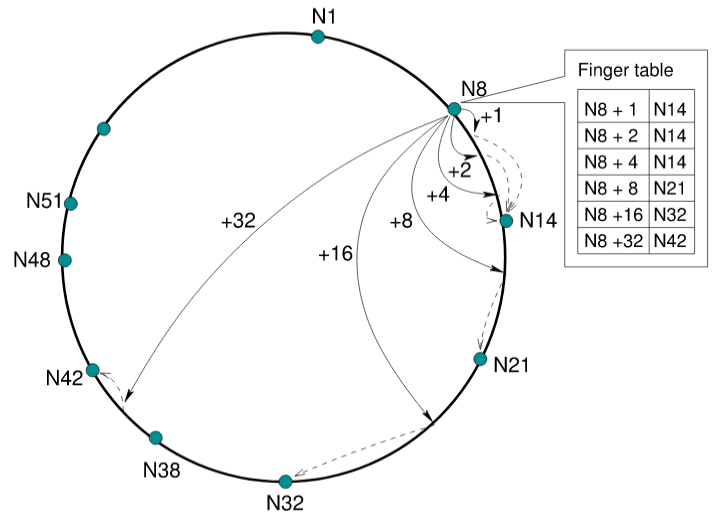
\includegraphics[scale=0.45]{chord.png}
	\centering
\end{figure}

\section{Distributed data processing}
Distributed databases are a great solution to optimize memory and speed, yet not every operation is supported by them. Machine learning or graph algorithms, for instance, are hard to compute on a sharded relational schema.

Analysis can be implemented in several different ways, but certain tasks need to be handled in every implementation:
\begin{itemize}
	\item Parallelization/synchronization;
	\item Distribution of computation and data;
	\item Communication between nodes;
	\item Node failures.
\end{itemize}

Creating a custom solution takes time and is error prone; functional abstractions can be used to specify computation in parallel. The runtime system, this way, manages program execution, data distribution and persistence, node failures and communication.

When a cluster is necessary, it is possible to use pre-configured structures:
\begin{enumerate}
	\item Infrastructure as a Service, externalizing resources and storage;
	\item Platform as a Service, renting databases and web servers;
	\item Software as a Service, using developer tools and additional packages.
\end{enumerate}

\subsection{MapReduce}
MapReduce is a programming model with associated implementation for processing and generating big data sets with a parallel distributed algorithm on a cluster.

It is composed of:
\begin{enumerate}
	\item A Map procedure, which performs filtering and sorting, applied by each worker to the local data and collecting output to a temporary storage;
	\item A Shuffle phase, where workers redistribute data based on the same output keys, so that all data with the same key is located on the same node;
	\item A Reduce method, which executes a summary operation (such as counting) on local data in parallel.
\end{enumerate}

The model is inspired by functional programming, but its key contributions are the scalability and fault tolerance achieved by optimizing the execution engine, especially on multi-threaded implementations. 

Maps can be performed in parallel, and a set of reducers can perform the reduction phase. Parallelism offers possibility of recovering from partial failure of servers or storage: the work can be rescheduled without recomputing all of it.

Logically, Map takes one pair of data with a type in one data domain, and returns a list of pairs in a different domain:
$$Map(k_1, v_1) \rightarrow list(k_2, v_2)$$

The Reduce function is then applied in parallel to each group, which in turn produces a collection of values in the same domain:
$$Reduce(k_2, list(v_2)) \rightarrow list((k_3, v_3))$$

Each Reduce call typically produces either one key-value par or an empty return.

Example (from Wikipedia):
\begin{lstlisting}
function map(String name, String document):
	// name: document name
	// document: document contents
	for each word w in document:
		emit (w, 1)

function reduce(String word, Iterator partialCounts):
	// word: a word
	// partialCounts: a list of aggregated partial counts
	sum = 0
	for each pc in partialCounts:
		sum += pc
	emit (word, sum)
\end{lstlisting}
This MapReduce performs a word count on a document. Each document is split into words, and every word is counted by Map; then all pairs with the same key are put together and sent to Reduce, which sums the relative counts.

MapReduce implementaton can be applied to many algorithms, such as joining of two relations or PageRank.

\subsubsection{PageRank}
PageRank is an algorithm used by Google Search to rank web pages in their search engine results, measuring the relevance of them.

It works assigning a numerical weight to each element of an hyperlinked set of documents, with the purpose of obtaining its relative importance within the set.

It outputs a probability distribution used to represent the likelihood that a person randomly clicking on links will arrive at any particular page. Links from a page to itself are ignored.

The PageRank transferred from a given page to the targets of its outbound links upon the next iteration is divided equally among all outbound links. 

The value for a page $v$ is dependent on the values for each page  in the set containing all pages linking to $v$, divided by the number of links from $v$.

Pseudo-code PageRank:
\begin{enumerate}
	\item Retrieve total number of nodes $n$;
	\item Write initial values in each node, computed as $\frac{1}{n}$;
	\item Find next node as $\frac{1-d}{n}$, where $d$ is the correction factor;
	\item For each iteration of the algorithm:
	\begin{enumerate}
		\item Compute outgoing page rank fraction;
		\item Add fraction to all neighbors;
	\end{enumerate}
	\item Swap next node and current;
	\item Reset next reassigning it the value of $\frac{1-d}{n}$.
\end{enumerate}

This algorithm looks at each node in the graph, computes the fraction of rank it has to pass on to neighbors, and writes it.

For better performance, the value can be computed in reverse, collecting all fractions from reverse neighbors.

The sequential reads are optimized for modern computers, but the random access to next node exhibits performance problems. Caches help alleviating this, since they can store most visited nodes.

If the memory requirements exceed the available main memory, the system will allocate too much memory, running into several page faults. Sorting by degree will make often-accessed nodes all in the same page.

The distributed version sends computed values to other nodes, but can cause overhead and network congestion. MapReduce assigns the Shuffle phase the duty of message passing.

Computing PageRank using MapReduce is also performed using the function to repeatedly multiply a vector by the matrix representing how the distribution changes after every single step.

\subsection{Hadoop}
Hadoop is an open-source implementation of the MapReduce framework, written in Java (opposed to the proprietary of Google in C++). It is now an Apache project used for very large clusters to handle big data sets.

\subsubsection{MapReduce}
Hadoop MapReduce is an application on the cluster that negotiates resources with YARN: a JobTracker globally manages jobs, and every node has its own TaskTracker.

\begin{enumerate}
	\item An user submits job configuration to JobTracker;
	\item JobTracker submits mapper tasks to TaskTrackers, scheduling computation on all available cluster nodes;
	\item Each task works on the data local to its node;
	\item The Shuffler moves output produced my Map among the nodes in the cluster;
	\item Once shuffling is complete, JobTracker schedules Reduce to all nodes.
\end{enumerate}

Since the datasets are much larger than the main memory and processing happens on very big clusters, intermediate results must be written to disk and shuffled results should be ordered.

MapReduce is however a framework not suitable for all uses: not everything can be expressed through the functions it offers, plus it is not a good fit for workloads with a lot of computation and smaller datasets.

\subsubsection{HDFS}
Hadoop relies on a distributed file system (HDFS), the primary data storage set used by its applications. It supports the rapid transfer of data between compute nodes, breaking information down into separate blocks and distributing it.

The file system ensures durability and data distribution, storing data read by Map, and pre-sorting and saving its output. 

Shuffling moves data between nodes and merges pre-sorted data, and results of Reduce are again written to HDFS.

HDFS is highly fault tolerant: the system replicates data multiple times, placing at least one copy on a different server rack than the others.

Files are split into blocks of 64MB, and by default each block has 3 replicas, so that missing data can be reconstructed. 

It follows a master-slave architecture: Name node manages file system and regulates access, while data nodes manage attached storage.

I/O is boosted by striping blocks of data over multiple disks, writing in parallel. HDFS exposes append-only files to users.

JobTracker is responsible to cope with failing nodes: it notices that one TaskTracker is not responsive, and its task gets reassigned to another node.

If its job is in Reduce phase, the correspondent function is restarted on other TaskTrackers.

\subsubsection{YARN}
YARN stands for Yet Another Resource Negotiator, and is a redesigned resource manager and large-scale distributed operating system for Hadoop.

YARN splits up the functionalities of resource management and job scheduling into separate daemons, to obtain a global resouce manager and a master for every application.

The ResourceManager and the NodeManager form the data computation framework. A NodeManager is the agent in every machine which is responsible for containers, monitoring their resource usage and reporting results to the ResourceManager.

The Scheduler is responsible for allocating resources to the various running applications subject to constraints such as capacity, performing no tracking of application status.

\subsection{Optimizations}
To optimize MapReduce it is possible to add a combiner, an optional class that operated by accepting input from Map and passing it to Reduce after summarizing records with the same key.

It operates on each Map output key, having the same key-value output as the Reducer, and it helps segregating data into multiple groups.

Folding is a function to save disk space: it analyzes a recursive data structure, and returns recombined results by recursively processing its constituent parts.

Programs working well on large clusters require a deep understanding of warehouse-sized computers: different settings need different techniques. In general, HDFS should be portable.

Overall, Hadoop considers hardware failure to be the norm, with applications needing streaming access on large datasets. Its model, therefore, uses a model aiming to minimize writes and keeps computation local with the data.

\subsection{Scale up vs. out}
A data center is usually made of computers piled in racks, and racks are connected via a switch to form a cluster.

Accessing data on remote machines comes with a price: the faster is a local DRAM (20GB/S), but cluster DRAMs and disks are relatively slow. 

In case no single machine is large enough to store all the data, it is necessary to choose between scaling up and out: a cluster of large expensive machines or a large cluster of cheap commodity machines.

A simple execution model calculates the total cost summing the expense of computation with all global data access. The data kept locally is inversely proportional to the size of cluster.
$$ TotalCost = \frac{1ms}{n} + f \times \Big[100ns \times \frac{1}{n} + 100\mu s \times \Big(1 - \frac{1}{n}\Big) \Big]$$

\begin{itemize}
	\item Light communication: $f = 1$;
	\item Medium communication: $f = 10$;
	\item Heavy communication: $f = 100$.
\end{itemize}

Workloads with light communication benefit from large clusters, while large amounts of random communication impede performance. Random reads must be avoided!

\subsection{Spark}
Spark is an alternative to Hadoop which provides more expressive fault-tolerant runtime for distributed batched data analytics. It can handle more complex analysis with interactive queries processing real time streams.

The purpose of a new programming model is extending the existing naive algorithms implementation:
\begin{itemize}
	\item Data can be outputted by sorted key;
	\item Locality can be increased using different kinds of partitioning;
	\item Window queries can be answered sorting by group.
\end{itemize}

The MapReduce model is extended too with complex data pipelines, but recovery mechanisms are lightweight and require less additional computation.

Sparks offers additional API for more functionalities, such as Spark SQL, GraphX and MLIB.

\subsubsection{RDDs}
Spark revolves around the concept of a resilient distributed dataset (RDD), which is a fault-tolerant collection of elements that can be operated on in parallel.

RDD is considered the evolution of the general Spark model, offering datasets that can be efficiently cached and manipulated. 

RDDs support two types of operations: transformations, which create a new dataset from an existing one, and actions, which return a value to the driver program after running a computation on the dataset.

All transformations in Spark are lazy, in that they do not compute their results right away. Instead, they just remember the transformations applied to some base dataset (e.g. a file). 

They are only computed when an action requires a result to be returned to the driver program, and the dataset gets only loaded when operations are performed on it. This design enables Spark to run more efficiently.

Pipelines allow to chain transformations and intermediate steps do not need to be materialized since they can just be recomputed on node failure.

\subsubsection{DataFrames}
DatFrames are dynamically strongly typed distributed collections of data organized into columns, conceptually equivalent to a table in a relational database.

They can be interacted with using SQL functions, allowing query optimization and avoiding interpretation overhead, although with a limited set of functions.

\subsubsection{Datasets}
A Dataset is a combination between DataFrame and RDD, optionally weakly typed, to retain code compilation. It is still mapped as a RDD.

Datasets can be created, analyzed (limited, filtered) and be subject of exploration, management or aggregation just like tables.

\subsubsection{Optimization}
RDDs track lineage information to rebuild lost data, logging everything in a graph to recompute missing or damaged partitions. Spark offers support for DAGs.

Snapshots are automatically created after repartitioning transformations and managed using a LRU cache to speed up recovery.

The optimizer builds a logical plan and applies transformation rules, to then generate the physical plan and select the cheapest cost model. 

Spark's runtime focuses on three main points:
\begin{itemize}
	\item Memory Management and Binary Processing, leveraging semantics to eliminate the overhead of deserialization and garbage collection;
	\item Cache-aware computation, using columnar storage and compression to exploit memory hierarchy;
	\item Code generation to optimize usage of modern compilers and CPU.
\end{itemize}

Operations to take care of reading, managing ETL pipelines, training and query are performed within the same framework.
